\chapter{Redes neuronales}
%\section{El perceptrón simple}
%\begin{imagen}
%	\scalebox{1.5}{\begin{tikzpicture}
	%\node [circle split, draw, rotate=90, inner sep=-1pt]  (neurona) at (0, 0) {\rotatebox{-90}{\scriptsize $\sum$} \nodepart{lower} \rotatebox{-90}{\scriptsize $f(z)$}};
	\node [circle, draw, inner sep=1pt] (neurona) at (0, 0) {\scriptsize $\sum_i w_{i}x_{i}$};

	\node (in_0) at (-2.5, 1.5) {$x_0$};
	\node (in_1) at (-2.5, 0.5) {$x_1$};
	\node (in_2) at (-2.5, -0.5) {$x_2$};
	\node (in_n) at (-2.5, -1.5) {$x_n$};
	\node (out) at (2.0, 0.0) {$y_0$};

	\node (d2) at ($(in_2)!0.5!(in_n)$) {$\mathbf{\vdots}$};


	\draw[->] (in_0) -- node[above, pos=0.40] {\scriptsize$w_0$} (neurona);
	\draw[->] (in_1) -- node[above, pos=0.40] {\scriptsize$w_1$} (neurona);
	\draw[->] (in_2) -- node[above, pos=0.40] {\scriptsize$w_i$} (neurona);
	\draw[->] (in_n) -- node[above, pos=0.40] {\scriptsize$w_n$} (neurona);
	\draw[->] (neurona) -- node[above] {$f$} (out);
\end{tikzpicture}
}
%	\caption{Perceptrón simple}
%	\label{fig:perceptron}
%\end{imagen}

\section{Las redes neuronales}
El elemento básico de las NN es el nodo, que recibe un vector de entrada para producir una salida como muestra en la figura \ref{fig:perceptron}. Cada entrada tiene asociado un vector de pesos $w$, que se va modificando durante el proceso de aprendizaje. Cada unidad aplica una función $f$ sobre la suma de las entradas ponderada por el vector de pesos como en la ecuacion \ref{eq:entrada}.
\begin{eqnarray}
	y_{i} = \sum_{j} w_{ij}y_{j}\label{eq:entrada}
\end{eqnarray}
Donde el resultado puede servir como entrada de otras unidades.

Existen dos fases importante dentro del modelo
\begin{itemize}
	\item Fase de entrenamiento: Se usa un conjunto de datos o patrones de entrenamiento para determinar los pesos que definen el modelo de la NN. Se calculan de manera iterativa, de acuerdo con los valores de entrenamiento, con el objeto de minimizar el error cometido entre la salida obtenida por la NN y la salida deseada.

	\item Fase de prueba: Durante el entrenamiento, el modelo se ajusta al conjunto de entrenamiento, perdiendo la habilidad de generalizar su aprendizaje a casos nuevos, a esta situación se le llama sobreajuste.
	Para evitar el sobreajuste, se utiliza un segundo grupo de datos diferentes, el conjunto de validación, que permitirá controlar el proceso de aprendizaje.
\end{itemize}
Los pesos óptimos se obtienen minimizando una función. Uno de los criterios utilizados es la minimización del error cuadrático medio entre el valor de salida y el valor real esperado.






\section{El perceptrón multicapa}
El perceptrón multicapa es una generalización del perceptrón simple, y surgió como consecuencia de las limitaciones de dicha arquitectura para resolver problemas de clasificación no lineal. \citeA{Minsky1969b} mostraron que el uso de varios perceptrones simples podía resultar una solución para resolver problemas no lineales. Sin embargo, dicha propuesta no presentaba una solución al problema de la actualización de los pesos de las capas, pues la regla de aprendizaje del perceptrón simple no era aplicable. Rummelhart, Hinton y Wilians presentaron la {\em regla delta generalizada}, una forma de propagar el error de la red desde la capa de salida hacia las capas anteriores.

Dentro de las redes neuronales, el perceptrón multicapa es una de las arquitecturas más usadas para resolver problemas. Esto es debido a que poseen la capacidad de ser un aproximador universal. Esto no implica que sea una de las redes más potentes o con mejores resultados, el perceptrón multicapa posee una serie de limitaciones, como el proceso de aprendizaje para problemas que dependan de un gran número de variables, la dificultad para realizar un análisis teórico de la red debido a la presencia de componentes no lineales y a la alta conectividad.

\subsection{Arquitectura}
El perceptron multicapa posee una estructura de capas compuestas por neuronas. Cada una de las capas está formada por un conjunto de neuronas y se distinguen tres tipos de capas: la capa de entrada, las capas ocultas y la capa de salida.

Las neurones de la capa de entrada se encargan de recibir los patrónes y propagar dichas señales a las neuronas de la capa siguiente. La última capa, la capa de salida, proporciona la respuesta de la red al patrón presentado. Las neuronas de las capas ocultas realizan el procesado de las señales generadas por el patrón de entrada.
\begin{imagen}
	\scalebox{0.8}{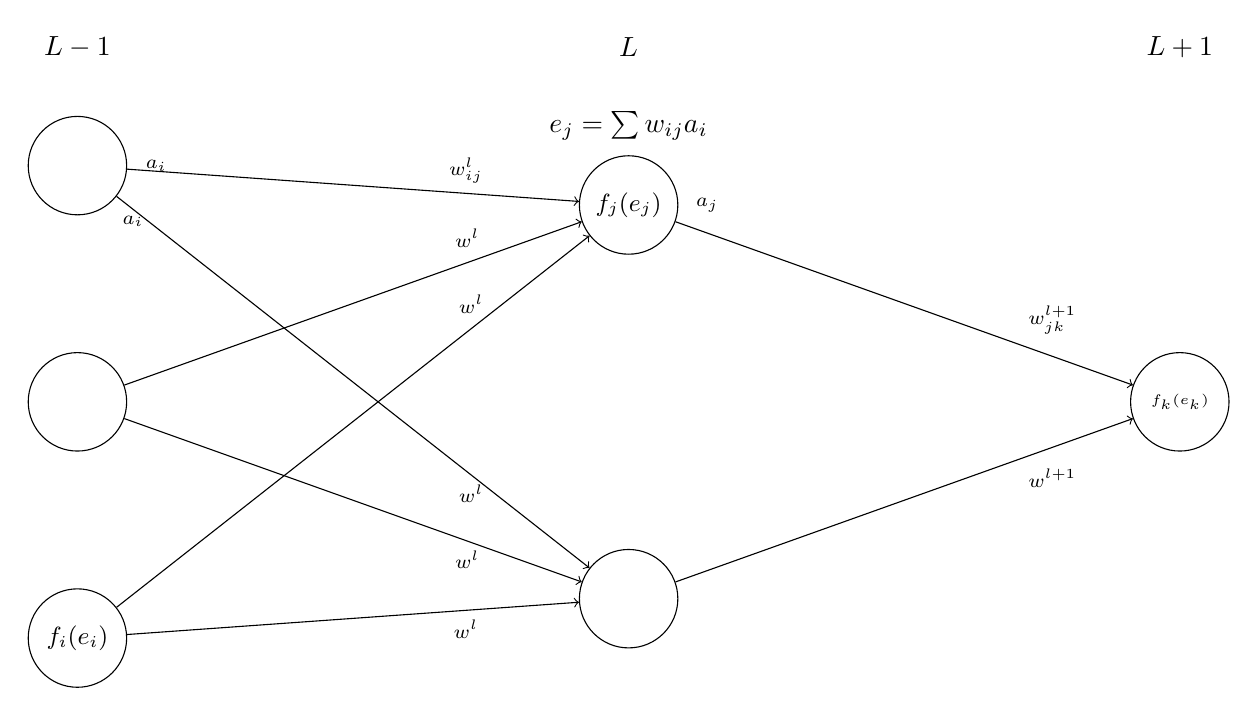
\begin{tikzpicture}

	\tikzstyle{nodo}=[circle, draw, minimum size=1.25cm]
	\tikzstyle{upw}=[dashed, red, ->, line width = 1pt]

	\coordinate (l_0) at (0, 4.5);
	\coordinate (l_1) at (7, 4.5);
	\coordinate (l_2) at (14, 4.5);

	\coordinate (f_1_1) at (0, 3); % CAPA ENTRADA
	\coordinate (f_1_2) at (0, 0); % CAPA ENTRADA
	\coordinate (f_1_3) at (0, -3); % CAPA ENTRADA
	\coordinate (f_2_1) at (7, 2.5); % CAPA OCULTA 1
	\coordinate (f_2_2) at (7, -2.5); % CAPA OCULTA 1
	\coordinate (f_3_1) at (14, 0); % CAPA SALIDA

	\node[] (l_0) at (l_0) {$L - 1$};
	\node[] (l_1) at (l_1) {$L$};
	\node[] (l_2) at (l_2) {$L + 1$};

	\node[nodo] (f_1_1) at (f_1_1) {}; % CAPA ENTRADA
	\node[nodo] (f_1_2) at (f_1_2) {}; % CAPA ENTRADA
	\node[nodo] (f_1_3) at (f_1_3) {\small $f_i(e_i)$}; % CAPA ENTRADA
	\node[nodo] (f_2_1) at (f_2_1) {\small $f_j(e_j)$}; % CAPA OCULTA 1
	\node[nodo] (f_2_2) at (f_2_2) {}; % CAPA OCULTA 1
	\node[nodo] (f_3_1) at (f_3_1) {\tiny $f_k(e_k)$}; % CAPA SALIDA


	\draw[->, font=\scriptsize] (f_1_1) node[right of=f_1_1] {$a_{i}$} -- node[pos=0.75, above] (w_1_1) {$w^{l}_{ij}$} (f_2_1);
	\draw[->, font=\scriptsize] (f_1_2) node[below right of=f_1_1] {$a_{i}$} -- node[pos=0.75, above] (w_1_2) {$w^{l}_{}$} (f_2_1);
	\draw[->, font=\scriptsize] (f_1_3) -- node[pos=0.75, above] (w_1_3) {\scriptsize$w^{l}_{}$} (f_2_1);
	\draw[->, font=\scriptsize] (f_1_1) -- node[pos=0.75, below] (w_2_1) {$w^{l}_{}$} (f_2_2);
	\draw[->, font=\scriptsize] (f_1_2) -- node[pos=0.75, below] (w_2_2) {$w^{l}_{}$} (f_2_2);
	\draw[->, font=\scriptsize] (f_1_3) -- node[pos=0.75, below] (w_2_3) {$w^{l}_{}$} (f_2_2);

	\node[above of=f_2_1] {$e_{j} = \sum w_{ij}a_i$};

	\draw[->, font=\scriptsize] (f_2_1) node[right of=f_2_1] {$a_{j}$} -- node[pos=0.75, above right] (w_j_k) {$w^{l+1}_{jk}$} (f_3_1);
	\draw[->, font=\scriptsize] (f_2_2) -- node[pos=0.75, below right] {$w^{l+1}$} (f_3_1);


	%\draw[upw] (f_3_1) to[bend left=20] (w_1_1);
	%\draw[upw] (f_3_1) to[bend left=20] (w_1_2);
	%\draw[upw] (f_3_1) to[bend left=20] node[pos=0.7, right] {$w^{l}_{ij} - \alpha\frac{\partial e}{\partial w}$} (w_1_3);


	%\draw[upw] (f_4_1) to[bend right=20] node[pos=0.8, right] {$w^{l+1}_{jk} - \alpha\frac{\partial e}{\partial w^{l+1}_{jk}}$} (w_j_k);

	%\node[above right of=w_j_k, node distance=3cm] {$\frac{\partial e}{\partial w^{l+1}_{jk}}=-(s_i - y_i)\frac{\partial y_i}{\partial w^{l+1}_{jk}}$};
\end{tikzpicture}
}
	\caption{Neurona}
	\label{fig:neurona}
\end{imagen}

En la figura \ref{fig:neurona} se observa que las conexiones van siempre hacia adelante, es decir, las neuronas de la capa $l$ se conectan con las neuronas de la capa $l + 1$. Las neuronas de una capa están conectadas a todas las neuronas de la capa siguiente.

\subsection{Propagación de la entrada}
El perceptrón multicapa define una relación entre la entrada y la salida. Esta relación se obtiene propagando hacia adelante los valores de las variables de entrada, es por esto que también se les llama redes {\em feedforward}. Cada neurona de la red procesa la entrada recibida y produce una respuesta que se propaga, mediante las conexiones, hacia las neuronas de la capa siguiente.

Si un perceptrón multicapa con $C$ capas y $n_c$ neuronas en la capa $c$, donde $W_c = (w^{c}_{ij})$ es la matriz de pesos, donde $w^{c}_{ij}$ representa el peso de la conexion de la neurona $i$ de la capa $c$. Denotaremos $a^{c}_{i}$ a la activación de la neurona $i$ de la capa $c$ que se calcula de la siguiente manera
\begin{itemize}
	\item Activación de una neurona de la capa de entrada: Las neuronas se encargan de transmitir la entrada recibida, por lo tanto $$ a^{1}_{i} = x_{i}, i = 1, 2, \cdots, n$$ donde $X = (x_1, x_2, \cdots, x_n)$ representa el vector de entrada.

	\item Activación de una neurona de la capa oculta: Las neuronas de una capa oculta procesa la información recibida aplicando la función de activación $f$ a la suma de los productos de la entrada por sus pesos, es decir $$ a^{c}_{i} = f\left(\sum^{n_{c - 1}}_{j=1} w^{c - 1}_{ji}a^{c - 1}_{j} + \theta^{c}_{i}\right), i = 1, 2, \cdots, n_c; c = 2, 3, \cdots, C - 1$$ donde $a^{c - 1}_{j}$ es la salida de la capa anterior a $c$.

	\item Activación de una neurona de la capa de salida: La activación de una neurona de la capa de salida viene dada por la función de activación $f$ aplicada a la suma de los productos de la entrada por sus pesos, es decir $$ y_{i} = a^{c}_{i} = f\left(\sum^{n_{c - 1}}_{j=1} w^{C - 1}_{ji}a^{C - 1}_{j} + \theta^{C}_{i}\right), i = 1, \cdots, n_c$$ donde $Y = (y_1, y_2, \cdots, y_{n_{c}})$ es el vector de salida.
\end{itemize}

La función $f$ es la función de activación de la neurona. Las funciones de activación mas utilizadas son la sigmoidal y la tangente hiperbólica, descritas en las escuaciones \ref{eq:sigm} y \ref{eq:tanh} respectivamente.
\begin{eqnarray}
	f_{sigm}(x) &=& \frac{1}{1+\exp(-x)}\label{eq:sigm}\\
	f_{tanh}(x) &=& \frac{1 - \exp(-x)}{1 + \exp(-x)}\label{eq:tanh}
\end{eqnarray}

Ambas funciones poseen como imagen intervalo de valores entre $[0, 1]$ y $[-1, 1]$ como se observa en la figura \ref{fig:funciones}.% y están descritas por las ecuaciones \ref{eq:sigm} y \ref{eq:tanh}.

\begin{imagen}
	\scalebox{1.0}{
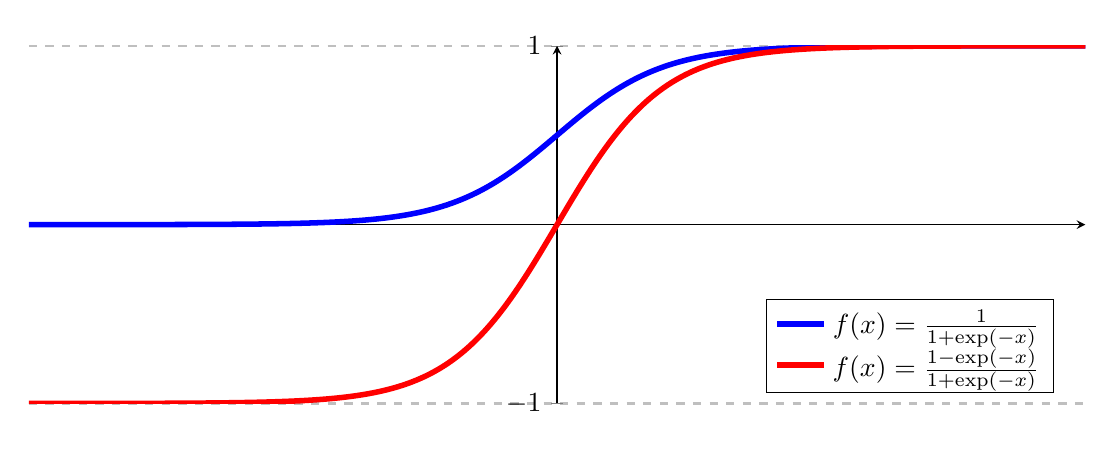
\begin{tikzpicture}
\begin{axis}[ymin=-1, ymax = 1, axis lines = left, legend pos=south east, width=15cm, xmajorticks=false, ytick={-1, +1}, axis lines=middle, y post scale=0.4, ymajorgrids=true, major grid style={dashed, line width=0.8pt}, yticklabel pos=left]
%Here the blue parabloa is defined
\addplot[domain=-10:10, samples=1000, color=blue, line width=2pt]{1/(1 + exp(-x))};
\addplot[domain=-10:10, samples=1000, color=red, line width=2pt]{(1 - e^(-x))/(1 + e^(-x))};
\addlegendentry{$f(x) = \frac{1}{1+\exp(-x)}$}
\addlegendentry{$f(x) = \frac{1 - \exp(-x)}{1 + \exp(-x)}$}
\end{axis}
%\begin{axis}[ymin=-1, ymax = 1, axis lines = left, xlabel = $x$, ylabel = {$f(x)$}]
%%Here the blue parabloa is defined
%\addplot[domain=-10:10, samples=1000, color=red]{(1 - e^(-x))/(1 + e^(-x))};
%\addlegendentry{$(1 - \exp(-x))/(1 + \exp(-x))$}
%\end{axis}
\end{tikzpicture}
% 1/(1+exp(-x))
}
	\caption{Funciones de activación mas utilizadas.}
	\label{fig:funciones}
\end{imagen}





\section{Algoritmo de retropropagación}
Una regla de aprendizaje es el método que le permite adaptar los parámetros de la red. El perceptrón multicapa actualiza sus pesos en función de la salida obtenida de tal manera que los nuevos pesos permitan reducir el error de salida. Por tanto, para cada patrón de entrada a la red es necesario disponer de un patrón de salida deseada.

El objetivo es que la salida de la red sea lo más próxima posible a la salida deseada, debido a esto la es que el aprendizaje de la red se describe como un problema de minimización de la siguiente maner $$ \min_{W} E $$ donde $W$ es el conjunto de parámetros de la red (pesos y umbrales) y $E$ es una función de error que evalúa la diferencia entre las salidas de la red y las salidas deseadas. en la mayor parte de los casos, la función de error se define como:
\begin{eqnarray}
	E = \frac{1}{N}\sum^{N}_{i = 1} e(i)
\end{eqnarray}

Donde $N$ es el número de muestras y $e(n)$ es el error cometido por la red para el patrón $i$, definido de la siguiente manera
\begin{eqnarray}
	e(i) = \frac{1}{n_{C}}\sum^{n_{C}}_{j = 1} (s_{j}(i) - y^{j}(n))^2\label{eq:error_patron}
\end{eqnarray}

Siendo $Y(i) = (y_{1}(i), y_{2}(i), \cdots, y_{n_{C}}(i))$ y $S(i) = (s_{1}(i), s_{2}(i), \cdots, s_{n_{C}}(i))$ los vectores de salida y salidas deseadas para el patrón $i$ respectivamente.

De esta manera, si $W^{*}$ es un mínimo de la función de error $E$, en dicho punto el error será cercano a cero, y en consecuencia, la salida de la red será próxima a la salida deseada.

Así es como el aprendizaje es equivalente a encontrar un mínimo de la función de error. La presencia de funciones de activación no lineales hace que la respuesta de la red sea no lineal respecto a los parámetros ajustables, por lo que el problema de aminimización es un problema no lineal y se hace necesario el uso de técnicas de optización no lineales para su resolución.

Las técnicas utilizadas suelen basarse en la actualización de los parámetros de la red mediante la determinación de una dirección de búsqueda. En el caso de las redes neuronales multicapa, la dirección de búsqueda más utilizada se basa en la dirección contraria del gradiente de la función de error $E$, el método de gradiente descendente.

Si bien el aprendizaje de la red busca minimizar el error total de la red, el procedimiento está basado en métodos del agradiente estocástico, que son una sucesión de minimizaciones del error en función de cada patrón $e(i)$, en lugar de minimizar el error total $E$ de la red. Aplicando el método del gradiente estocástico, cada parámetro $w$ se modifica para cada patrón de entrada $n$ según la siguiente regla de aprendizaje
\begin{eqnarray}
	w(i) = w(n - 1) - \alpha\frac{\partial e(i)}{\partial w}
\end{eqnarray}

donde $e(i)$ es el error para el patrón de entrada $i$ dado por la ecuación \ref{eq:error_patron}, y $\alpha$ es la tasa de aprendizaje, éste último determina el desplazamiento en la superficie del error.

Como las neuronas están ordenadas por capas y en distintos niveles, es posible aplicar el método del gradiente de forma eficiente, resultando en el {\em algoritmo de retropropagación} \cite{Rumelhart1986} o {\em regla delta generalizada}. El término retropropagación es utilizado debido a la forma de implementar el método del gradiente en las redes multicapa, pues el error cometido en la salida de la red es propagado hacia atrás, transformándolo en un error para cada una de las neuronas ocultas de la red.






% Neural Networks for Pattern Recognition - Bishop: 140 - Error backpropagation.
% Neural Networks for Pattern Recognition - Bishop: 263 - Gradient descent.
El algoritmo de retropropagación es el método de entrenamiento más utilizado en redes con conexión hacia adelante. Es un método de aprendizaje supervisado de gradiente descendente, en el que se distinguen claramente dos fases:
\begin{enumerate}
	\item Se aplica un patrón de entrada, el cual se propaga por las distintas capas que componen la red hasta producir la salida de la misma. Esta salida se compara con la salida deseada y se calcula el error cometido por cada neurona de salida.

	\item Estos errores se transmiten desde la capa de salida, hacia todas neuronas de las capas anteriores \cite{Fritsch1996}. Cada neurona recibe un error que es proporcional a su contribución sobre el error total de la red. Basándose en el error recibido, se ajustan los errores de los pesos sinápticos de cada neurona.
\end{enumerate}








%\section{Reglas de aprendizaje}
\section{El gradiente descendente}% http://alejandrosanchezyali.blogspot.cl/2016/01/algoritmo-del-gradiente-descendente-y.html
\begin{comment}
El gradiente descendente busca los punto $p \in \Omega$ donde funciones del tipo $f: \Omega\subseteq\mathbb{R}^m \rightarrow \mathbb{R}$ alcanzan su mínimo. La idea de este método se basa en que si $f$ es una función diferenciable en todo su dominio $\Omega$, entonces la derivada de $f$ es un punto $p \in \Omega$ en dirección de un vector unitario $v \in \mathbb{R}^m$ se define como

$$ df_{p}(v) = \nabla f(p)v $$

Observe que la magnitud de la ecuación es
$$ |d f_{p}(v)| = ||\nabla f(p)|| ||v||\cos\theta = ||\nabla f(p)\cos\theta$$

Dicha magnitud es máxima cuando $\theta = 2n\pi, n \in \mathbb{Z}$. Es decir, para que $|df_{d}(v)|$ sea máxima, los vectores $\nabla f(p)$ y $v$ debe ser paralelo. De esta manera, la función $f$ crece más rápidamente en la dirección del vector $\nabla f(p)$ y decrece más rápidamente en la dirección del vectro $-\nabla f(p)$. Dicha situación sugiere que la dirección negativa del gradiente $-\nabla f(p)$ es una buena dirección de búsqueda para encontrar el minimizador de la función $f$.

Sea $f: \Omega \subseteq \mathbb{R} \rightarrow \mathbb{R}$, si $f$ tiene un mínimo en $p$, para encontrar a $p$ se construye una sucesión de punto $\{p_{t}\}$ tal que $p_{t}$ converge a $p$. Para resolver esto, comenzamos en $p_{t}$ y nos desplazamos una cantidad $-\lambda_{t}\nabla f(p_{t})$ para encontrar el punto $p_{t + 1}$ más cercano a $p$, es decir:
$$ p_{t + 1} =p_{t} - \lambda _{t}\nabla f(p_{t}) $$

donde $\lambda_{t}$ se selecciona de tal manera que $p_{t + 1} \in \Omega$ y $f(p_{t}) \geq f(p_{t + 1})$

El parámetro $\lambda_{t}$ se seleccionara para maximizar la cantidad a la que decrece la función $f$ en cada paso.
\end{comment}

% http://neuralnetworksanddeeplearning.com/chap5.html
% ME ESTOY BASANDO EN : [1998b] Hochreiter
\subsection{El desvanecimiento del gradiente}
El problema del gradiente desvaneciente nace en las NN profundas, éstas utilizan funciones cuyo gradiente tienden a estar entre 0 y 1. Debido a que estos gradientes pequeños se multiplican durante la retropropagación, tienden a {\em desvanecerse} a través de las capas, evitando que la red aprenda en redes muy profundas.

%%%% VER QUE LA NOTACIÓN SEA COMPATIBLE
Si se tiene una NN, la activación de una neurona de una capa intermedia $i$ con función de activación $f_i$ y con entrada $$ net_{i}(t) = \sum_{j}w_{ij}y^{j}(t - 1) $$ es $y^{i}(t) = f_{i}(net_{i}(t))$. Además $w_{ij}$ es el peso de la conexión desde la unidad $j$ hasta la unidad $i$, $d_{k}(t)$ será la respuesta esperada de la unidad $k$ de la capa de salida en el tiempo $t$. Usando el error cuadrático medio ({\em Mean square error}, MSE), el error de $k$ será
$$ E_{k}(t) = (d_{k}(t) - y^{k}(t))^2 $$

En un tiempo $\tau \leq t$ cualquiera, el error de una neurona $j$ que no sea una neurona de entrada es la suma de los errores externos y el error propagado hacia atrás desde la neurona previa será
$$ \vartheta_{j}(\tau) = f'_{j}(net_{j}(\tau))\left(E_{j}(\tau) + \sum_{i} w_{ij}\vartheta_{i}(\tau + 1)\right) $$

El peso actualizado en el tiempo $\tau$ resulta
$$ w_{jl}^{new} = w_{jl}^{old} + \alpha\vartheta_{j}(\tau) y^{l}(\tau - 1)$$
donde $\alpha$ es la tasa de aprendizaje, y $l$ es una unidad arbitraria conectada a la unidad $j$.

En un tiempo arbitrario $\tau \leq t$, el error de la señal en una unidad $j$, que no sea de entrada, será la suma de los errores externos y la señal propagada anterioremente como muestra la ecuación \ref{eq:propagation_error}.
\begin{eqnarray}
	\vartheta(\tau) &=& f'_{j}(net_{j}(\tau)) \left(E_{j}(\tau) + \sum_{i}w_{ij}\vartheta_{i}(\tau + 1)\right)
	\label{eq:propagation_error}
\end{eqnarray}

Entonces, los pesos actualizados serán $$ w_{jl}^{new} = w_{jl}^{old} + \alpha\vartheta_{j}(\tau)y^{l}(\tau - 1) $$
\begin{comment}
Error en el factor de escala. Véase también las contribuciones anteriroes al análisis del desvanecimiento del gradiente \cite{Hochreiter1997a, Bengio1994, Hochreiter1991}. Propagando el error de una unidad $u$ en el timpo $t$ hacia una unidad $v$ {\Huge for $q$ time steps}, el error escala como muestra la ecuación \ref{eq:scale_error}
\begin{eqnarray}
	\frac{\partial \vartheta_{v}(t - q)}{\partial \vartheta_{u}(t)}
	&=&
	\left\{
	\begin{array}{lr}
		f'_{v}(net_{v}(t - 1))w_{uv}&q=1\\
		\\
		f'_{v}(net_{v}(t - q))\sum^{n}_{l = 1}\frac{\partial \vartheta_{l}(t - q + 1)}{\partial \vartheta_{u}(t)}w_{lv}	&q > 1
	\end{array}
	\right.\label{eq:scale_error}
\end{eqnarray}
\end{comment}

\begin{imagen}
	\scalebox{1.0}{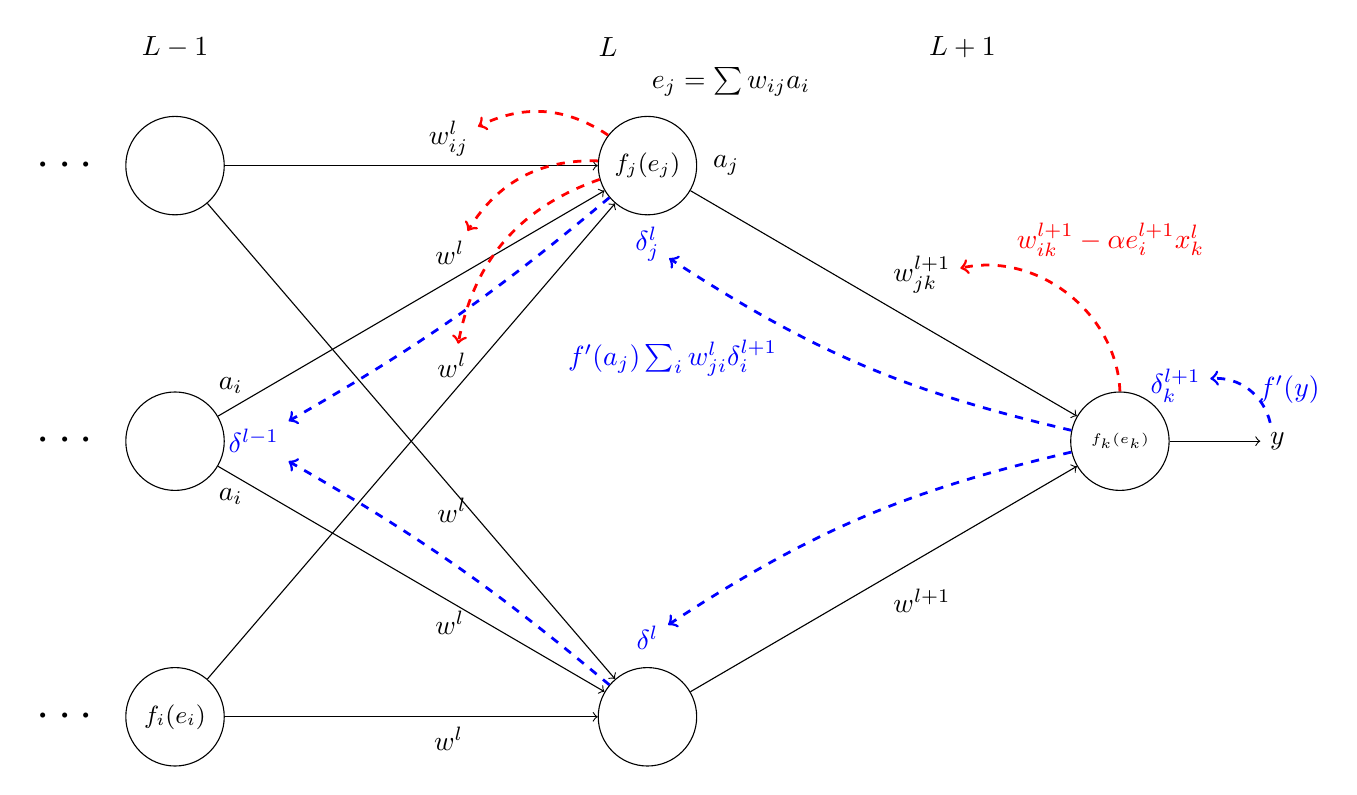
\begin{tikzpicture}

	\tikzstyle{nodo}=[circle, draw, minimum size=1.25cm]
	\tikzstyle{upw}=[dashed, red, ->, line width = 1pt]

	\coordinate (l_0) at (0, 5.0);
	\coordinate (l_1) at (5.5, 5.0);
	\coordinate (l_2) at (10, 5.0);

	\coordinate (f_1_1) at (0, 3.5); % CAPA ENTRADA
	\coordinate (f_1_2) at (0, 0); % CAPA ENTRADA
	\coordinate (f_1_3) at (0, -3.5); % CAPA ENTRADA
	\coordinate (f_2_1) at (6.0, 3.5); % CAPA OCULTA 1
	\coordinate (f_2_2) at (6.0, -3.5); % CAPA OCULTA 1
	\coordinate (f_3_1) at (12, 0); % CAPA SALIDA
	\coordinate (y) at (14, 0); % CAPA SALIDA

	\node[] (l_0) at (l_0) {$L - 1$};
	\node[] (l_1) at (l_1) {$L$};
	\node[] (l_2) at (l_2) {$L + 1$};

	\node[nodo] (f_1_1) at (f_1_1) {}; % CAPA ENTRADA
	\node[nodo] (f_1_2) at (f_1_2) {}; % CAPA ENTRADA
	\node[nodo] (f_1_3) at (f_1_3) {\small $f_i(e_i)$}; % CAPA ENTRADA
	\node[nodo] (f_2_1) at (f_2_1) {\small $f_j(e_j)$}; % CAPA OCULTA 1
	\node[nodo] (f_2_2) at (f_2_2) {}; % CAPA OCULTA 1
	\node[nodo] (f_3_1) at (f_3_1) {\tiny $f_k(e_k)$}; % CAPA SALIDA
	\node[] (y) at (y) {$y$}; % CAPA SALIDA

	\node[left of=f_1_1, node distance=1.4cm] {\LARGE $\cdots$};
	\node[left of=f_1_2, node distance=1.4cm] {\LARGE $\cdots$};
	\node[left of=f_1_3, node distance=1.4cm] {\LARGE $\cdots$};

	\draw[->] (f_1_1) -- node[pos=0.6, above] (w_1_1) {$w^{l}_{ij}$} (f_2_1);
	\draw[->] (f_1_2) -- node[pos=0.6, above] (w_1_2) {$w^{l}_{}$} (f_2_1);
	\draw[->] (f_1_3) -- node[pos=0.6, above] (w_1_3) {$w^{l}_{}$} (f_2_1);
	\draw[->] (f_1_1) node[above right of=f_1_2] {$a_{i}$} -- node[pos=0.6, below] (w_2_1) {$w^{l}_{}$} (f_2_2);
	\draw[->] (f_1_2) node[below right of=f_1_2] {$a_{i}$} -- node[pos=0.6, below] (w_2_2) {$w^{l}_{}$} (f_2_2);
	\draw[->] (f_1_3) -- node[pos=0.6, below] (w_2_3) {$w^{l}_{}$} (f_2_2);
	\draw[->] (f_2_1) node[right of=f_2_1] {$a_{j}$} -- node[pos=0.5, above right] (w_j_k) {$w^{l+1}_{jk}$} (f_3_1);
	\draw[->] (f_2_2) -- node[pos=0.5, below right] {$w^{l+1}$} (f_3_1);
	\draw[->] (f_3_1) -- node[pos=0.5, below right] {$$} (y);

	\node[above right of=f_2_1, node distance=1.5cm] {$e_{j} = \sum w_{ij}a_i$};


	\draw[upw] (f_3_1) to[bend right=50] node[above right, pos=0.8] {$w^{l+1}_{ik} - \alpha e^{l+1}_{i}x^{l}_{k}$} (w_j_k);
	\draw[upw] (f_2_1) to[bend right=30] node[above]{$$} (w_1_1);
	\draw[upw] (f_2_1) to[bend right=30] node[above]{$$} (w_1_2);
	\draw[upw] (f_2_1) to[bend right=30] node[above]{$$} (w_1_3);


	\node[blue, above right of=f_3_1] (e_i) {$\delta^{l+1}_{k}$};
	\node[blue, below of=f_2_1] (e_2_1_i) {$\delta^{l}_{j}$};
	\node[blue, above of=f_2_2] (e_2_2_i) {$\delta^{l}$};
	\node[blue, right of=f_1_2] (e_1_2_i) {$\delta^{l-1}$};

	\draw[upw, blue] (y) to[bend right=40] node[right]{$f'(y)$} (e_i);
	\draw[upw, blue] (f_3_1) to[bend left=10] node[below left, pos=0.7]{$f'(a_{j})\sum_{i}w^{l}_{ji}\delta^{l+1}_{i}$} (e_2_1_i);
	\draw[upw, blue] (f_3_1) to[bend right=10] (e_2_2_i);

	\draw[upw, blue] (f_2_1) to[bend left=5] (e_1_2_i);
	\draw[upw, blue] (f_2_2) to[bend right=5] (e_1_2_i);

\end{tikzpicture}
}
	\label{fig:vanishing}
	\caption{Gradiente descendente}
\end{imagen}
